\documentclass[../../main.tex]{subfiles}


\begin{document}

\subsection{Motivation}

%Each report must be created in a separate subfolder. Take the "example" folder as an example of a report (please do not change).
%
%Here it is required to describe the problematic of the problem. Basic premises and results. It is important to indicate a list of references on this topic~\cite{AuthorYear}. All refernces put to the main.bib file.
%
%After writing your report, include the report to main.tex similar to the sample report.

%All changes are made through GitHub\footnote{\url{https://github.com/Intelligent-Systems-Phystech/GeometricDeepLearning}}.

The work investigates the problem of time series forecasting. The goal is to get a continuous forecast given discrete data points.

\subsection{Problem statement}

Given a time series $\mathbf{X} = (t_i, a_i)^{\ell}_{i=1}, ~t_1 \leq \ldots \leq t_\ell$. The number $a_i$ is the accelerometer reading. Given also unobservable velocities $v_i \in \mathbb{R}^1$ at each timestamp $t_i$. The current velocity $v_i$ can be computed through the previous one as follows: $v_i = f(v_{i-1},a_{i}, \boldsymbol\theta_\text{rnn})$. It is assumed that at each interval $[t_{i-1}, t_i]$ the pendulum equation is fulfilled:
\[
\begin{cases}
\frac{d}{dt}a(t) = v(t),\\
\frac{d}{dt}v(t) = -\theta\sin a(t), \quad \theta > 0,\\
a(t_{i-1}) = a_{i-1} + \xi_{i-1}, ~v(t_{i-1}) = v_{i-1}.
\end{cases} \quad 2 \leq i \leq \ell
\]
Let $\boldsymbol\theta = [\theta, \boldsymbol\theta_\text{rnn}]$. Given a loss function $\mathcal{L}(\boldsymbol{\theta}) = \sum_{i=2}^\ell\xi_i^2(\boldsymbol\theta)$. Optimal parameters $\boldsymbol\theta$ are solution of the following optimization problem:
\[
\boldsymbol{\theta}^* = \arg\min_{\boldsymbol{\theta}}\mathcal{L}(\boldsymbol{\theta}).
\]

\subsection{Problem solution}
Consider basic algorithm ODE-RNN \cite{NEURIPS2019_42a6845a}:
\begin{algorithm}[H]
\begin{algorithmic}
\caption{ODE-RNN}
\REQUIRE Data points $\{(x_i, t_i)\}_{i=1}^N$.
\STATE Initialize $\mathbf{h}_0$.
\FOR{$i = 1, \ldots, N$}
\STATE $\mathbf{h}_i' = \mathrm{ODESolve}(f_\theta, \mathbf{h}_{i-1}, (t_{i-1}, t_i))$.
\STATE $\mathbf{h}_i = \mathrm{RNNCell}(\mathbf{h}_i', x_i)$.
\ENDFOR
\STATE For each $i$ compute outputs $o_i = \mathrm{OutputNN}(\mathbf{h}_i)$.
\RETURN $\{o_i\}_{i=1}^N$
\end{algorithmic}
\end{algorithm}

We introduce a modification of ODE-RNN. The difference is that we map hidden state to the space (from $\mathbb{R}^\text{hidden}$) of the ODE solution ($\mathbb{R}^2$) and back.
\begin{algorithm}[H]
\begin{algorithmic}
\caption{ODE-RNN with modifications}
\REQUIRE Data points $\{(x_i, t_i)\}_{i=1}^N$.
\STATE Initialize $\mathbf{h}_0$.
\FOR{$i = 1, \ldots, N$}
\STATE $\mathbf{h}_i' = \mathrm{ODESolve}(f_\theta, \textcolor{red}{\mathrm{To2d}}(\mathbf{h}_{i-1}), (t_{i-1}, t_i))$.
\STATE $\mathbf{h}_i = \mathrm{RNNCell}(\textcolor{red}{\mathrm{ToHidden}}(\mathbf{h}_i'), x_i)$.
\ENDFOR
\STATE For each $i$ compute outputs $o_i = \mathrm{OutputNN}(\mathbf{h}_i)$.
\RETURN $\{o_i\}_{i=1}^N$
\end{algorithmic}
\end{algorithm}

We compute gradients of the loss function $\mathcal{L}(\boldsymbol{\theta})$ w.r.t. $\boldsymbol\theta$ using backpropagation. Then we perform optimizing step. After some iterations we get a solution. 

\subsection{Code analysis}

The computational experiment can be found on GitHub repository\footnote{https://github.com/Konstantin-Iakovlev/MathMethodsOfForecasting}.

\subsection{Computational experiment}

The goal of the computational experiment is to compare the prediction quality of the proposed method with other methods. The data was taken from WISDM dataset \cite{kwapisz2011activity}. We considered an accelerometer measurements. The number of train timestamps is 60. The number of validation timestamps is 20. Hidden size of LSTM is 20. Output network, networks that map to hidden space and back are one layer dense networks.

First, we ran ODE-RNN with modifications with $f_\theta$ as a right hand side of a pendulum equation. We used Adam with learning rate $5\cdot 10^{-3}$ for optimization. We ran 500 epochs of optimization. Validation loss is 0.6090.

\begin{figure}[H]
\centering
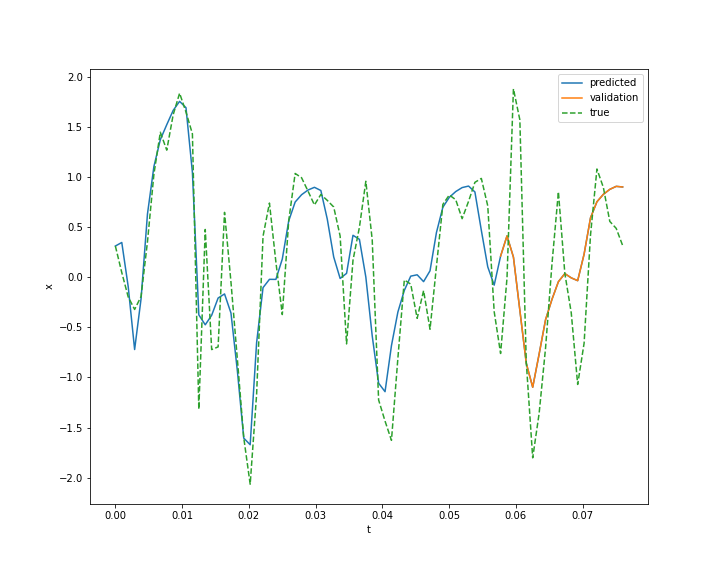
\includegraphics[width=0.8\textwidth]{figures/pendulum.png}
\caption{Forecast of ODE-RNN with modifications, pendulum equation.}
\end{figure}

After that we ran ODE-RNN with modifications with $f_\theta$ as a two fully connected layers with Tanh activation with hidden size 2. We also ran 500 epochs with Adam optimizer. The validation loss is 1.3758.


\begin{figure}[H]
\centering
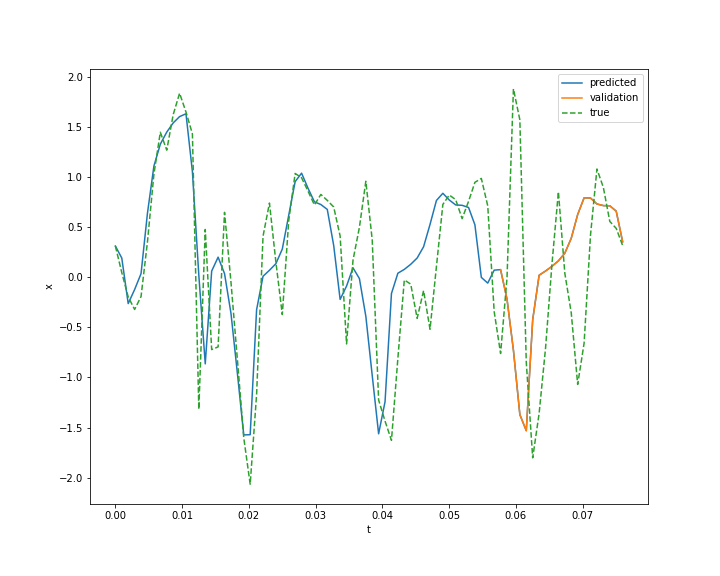
\includegraphics[width=0.8\textwidth]{figures/dense.png}
\caption{Forecast of ODE-RNN with modifications,  dense network.}
\end{figure}


\begin{figure}[H]
\centering
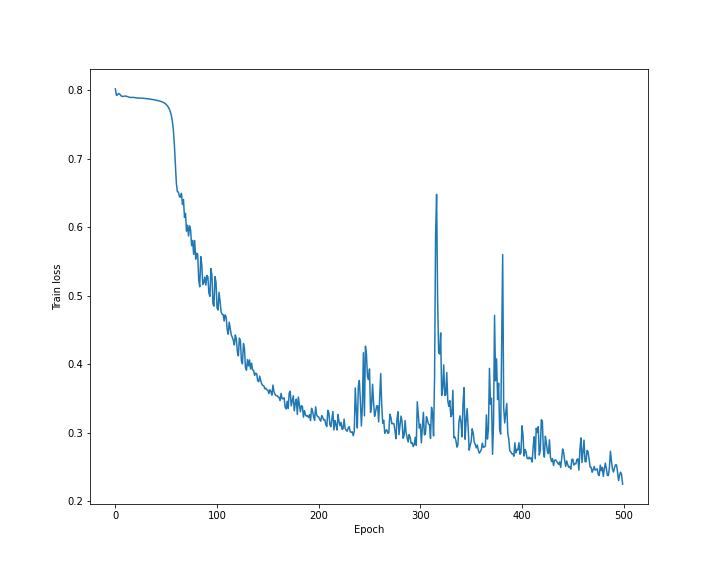
\includegraphics[width=0.8\textwidth]{figures/pendulum_train.png}
\caption{Train loss, pendulum equation.}
\end{figure}


\begin{figure}[H]
\centering
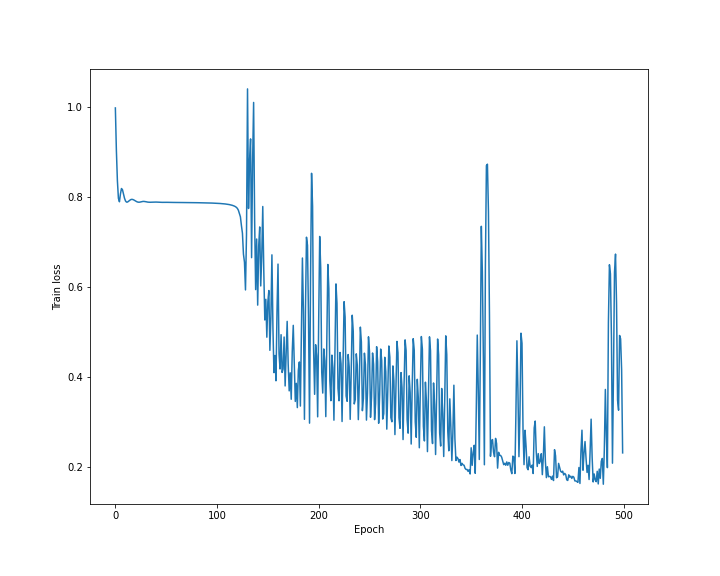
\includegraphics[width=0.8\textwidth]{figures/dense_train.png}
\caption{Train loss, dense network.}
\end{figure}

During our experiments, we noticed that the learning process of the network in the case of a pendulum is more stable and reach better minimum. It seems to be that the using of the pendulum equation's right hand side as a dynamic of an ODE is a powerful regularizer.
%\begin{table}
%\caption{Dependence of $Q^2$ on $R$ on validation dataset}
%\label{table}
%\begin{tabular}{c|c|c|c|c|c|c|c|}
%Method & $R= 1$ & $R= 4$ & $R = 10$ & $R = 13$ & $R = 16$ & $R = 19$\\ \hline
%HOPLS  &0.41 $\pm$ 0.12 & 0.51 $\pm$ 0.19&  0.41 $\pm$ 0.12& 0.04 $\pm$ 0.47 & -0.22 $\pm$ 0.68&  -0.32 $\pm$ 0.68 \\
%N-PLS & 0.42 $\pm$ 0.15 & 0.45 $\pm$ 0.11 & 0.35 $\pm$ 0.18 & 0.35 $\pm$ 0.19 & 0.33 $\pm$ 0.20 & 0.30 $\pm$ 0.20    
%\end{tabular}
%\end{table}



\end{document}